\section{Implementation of Scratch Detector}
In this chapter the development and results of a YOLOv5 solution for detection of scratches found on printed layers of a 3D binder jet printer.
\subsection{Development Environment \& Setup}
Through trial and error the development environment has been continuously improved and finally converged to the one depicted in figure \ref{fig:setup}. A simple dataset manager is used for dataset versioning through FiftyOne's \cite{fiftyone_git} integrated database. Datasets stored in FiftyOne's database can be then visualized in any browser. This helpful for debugging and testing new augmentations methods or visualizing detections and labels in a more interactive way. For annotating labels, CVAT \cite{cvat_git} was one of the more established tools for this task. \\
The augmentation of data can happen in two ways: offline and online. Ideally is to have as many online augmentations as possible, but the online augmentation framework provided by YOLOv5 forces that each augmentation method takes as input a exactly one labeled image and outputs exactly one labeled image. Changing this framework to be flexible to more output images is difficult, since the underlying albumentations library \cite{albumentations_site} works on the same one input-one output principle. Therefore, for those type of augmentations method is best to be made offline and this is the task of the \textit{Augmenter} from the figure. \\
For logging Weights \& Biases \cite{wandb_site} was a good candidate, because it's feature rich and YOLOv5 has native support for this. YOLOv5 supports also Tensorboard and ClearML.\\

 \begin{figure}[!h]
  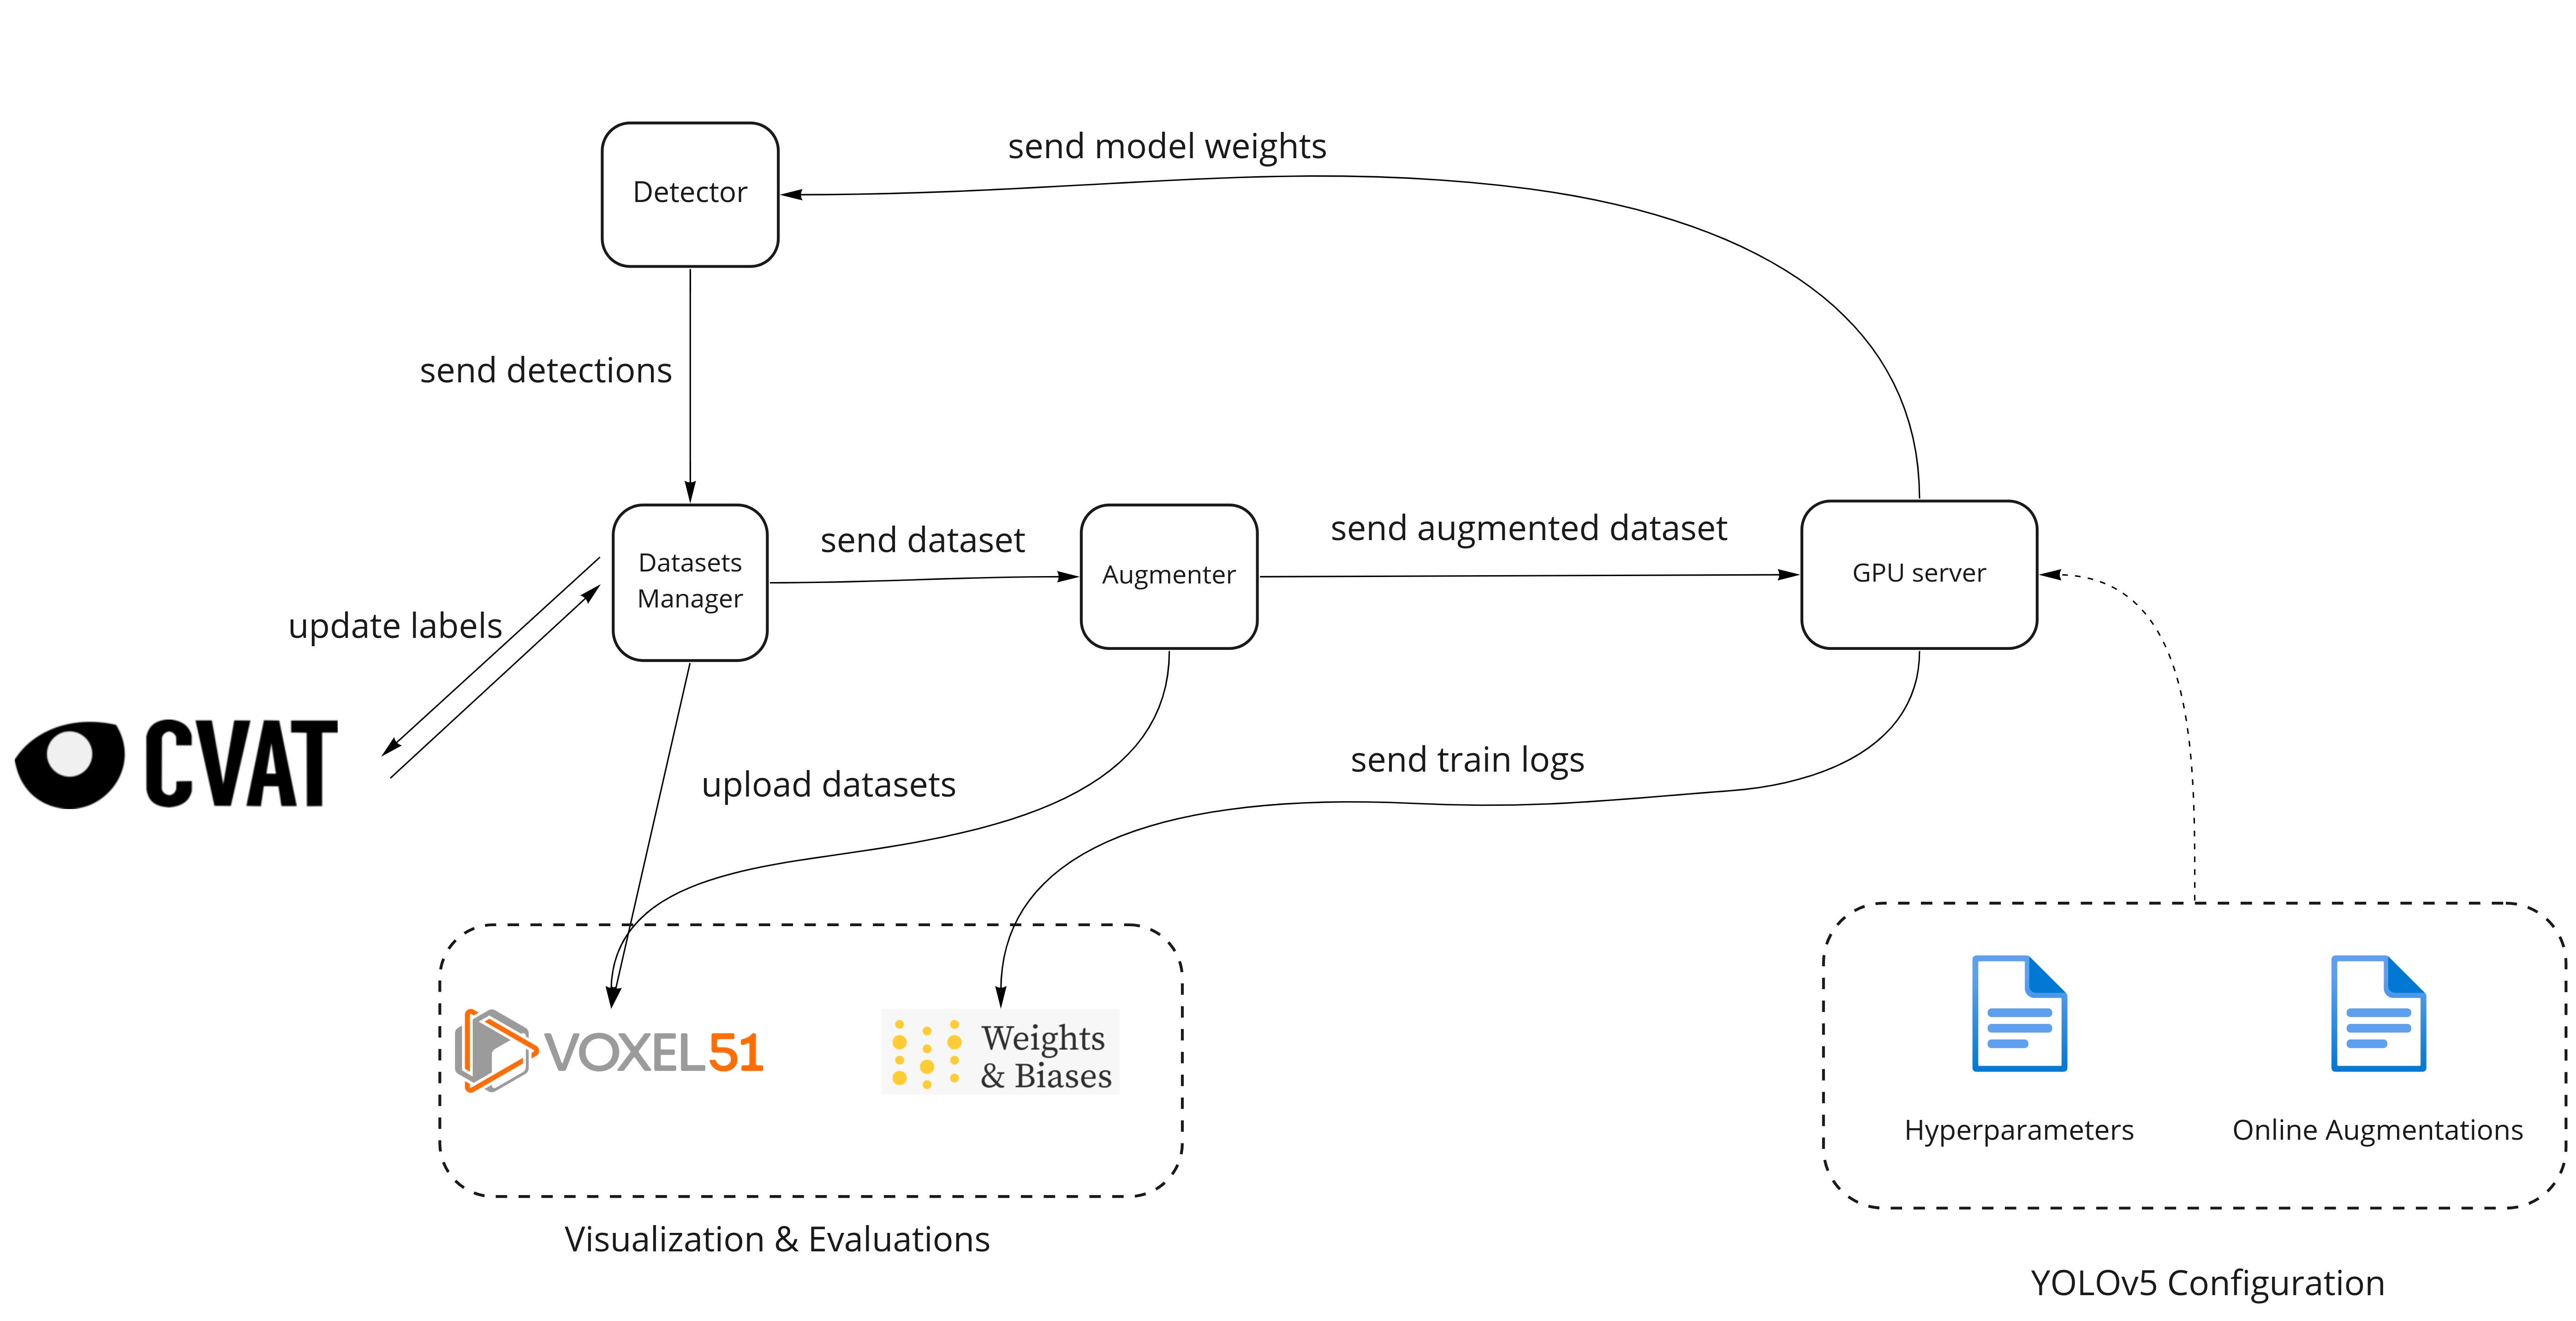
\includegraphics[width=\textwidth]{images/setup}
  \caption{title}
  \label{fig:setup}
\end{figure}

For detection the \textit{detector.py} script provided in YOLOv5 can be used, but an official detector can also be loaded from PyTorch Hub. The latter solution is better for post processing detections.

\subsection{Annotation}
Annotating the dataset was a tougher challenge than anticipated, because it's not always clear if the dark line is a scratch, thin split in the component or some artifact visible from the layer before. \\

\begin{figure}[ht]
  \centering

  \begin{subfigure}{\textwidth}
    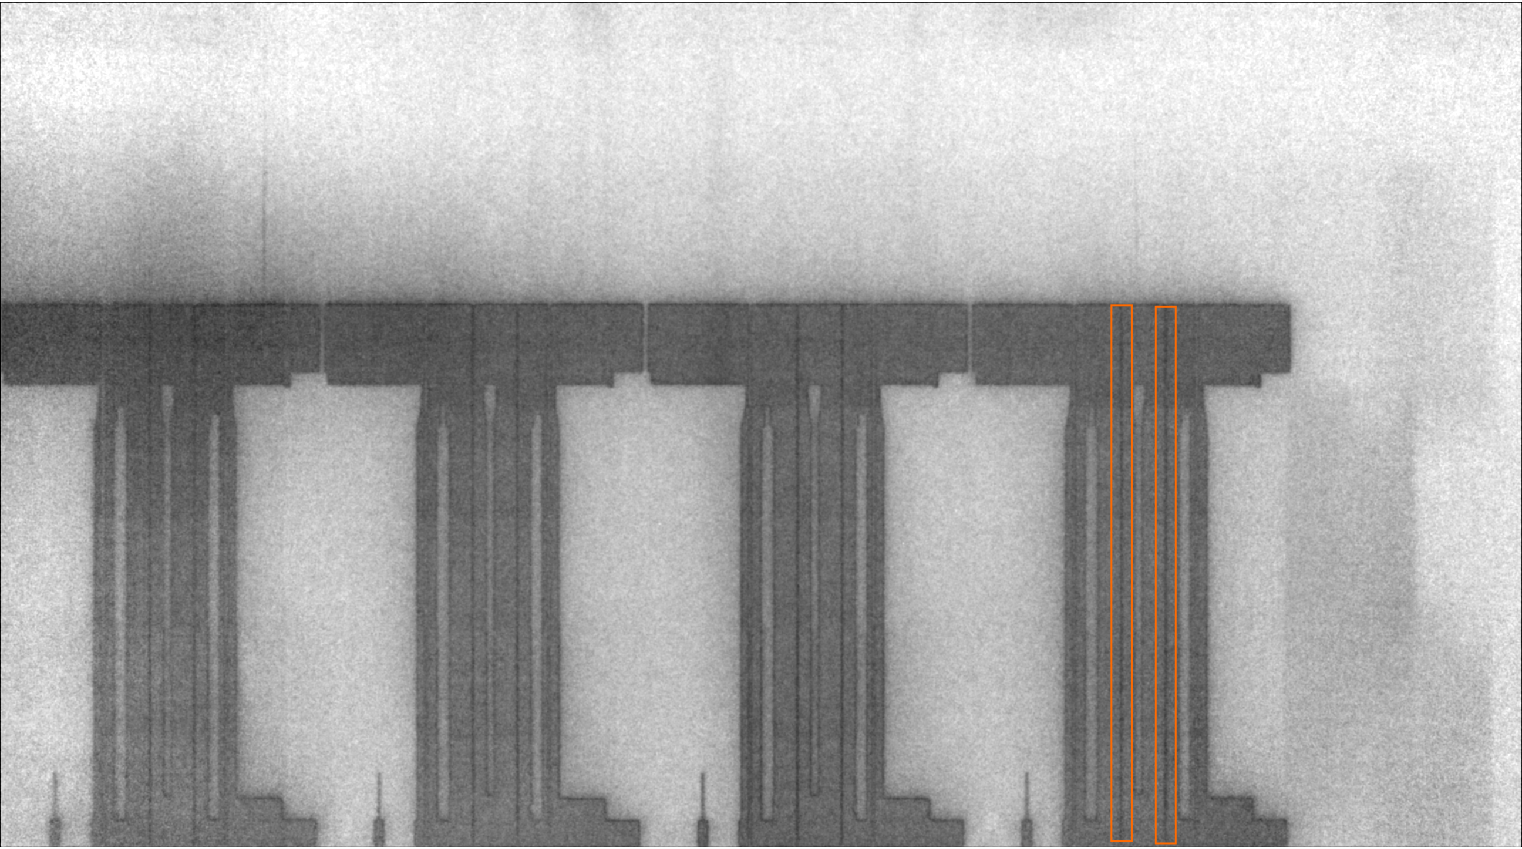
\includegraphics[width=\textwidth]{images/layer_01486_marked}
    \caption{Layer with thin splits marked in orange bounding boxes.}

  \end{subfigure}

  \begin{subfigure}{\textwidth}
    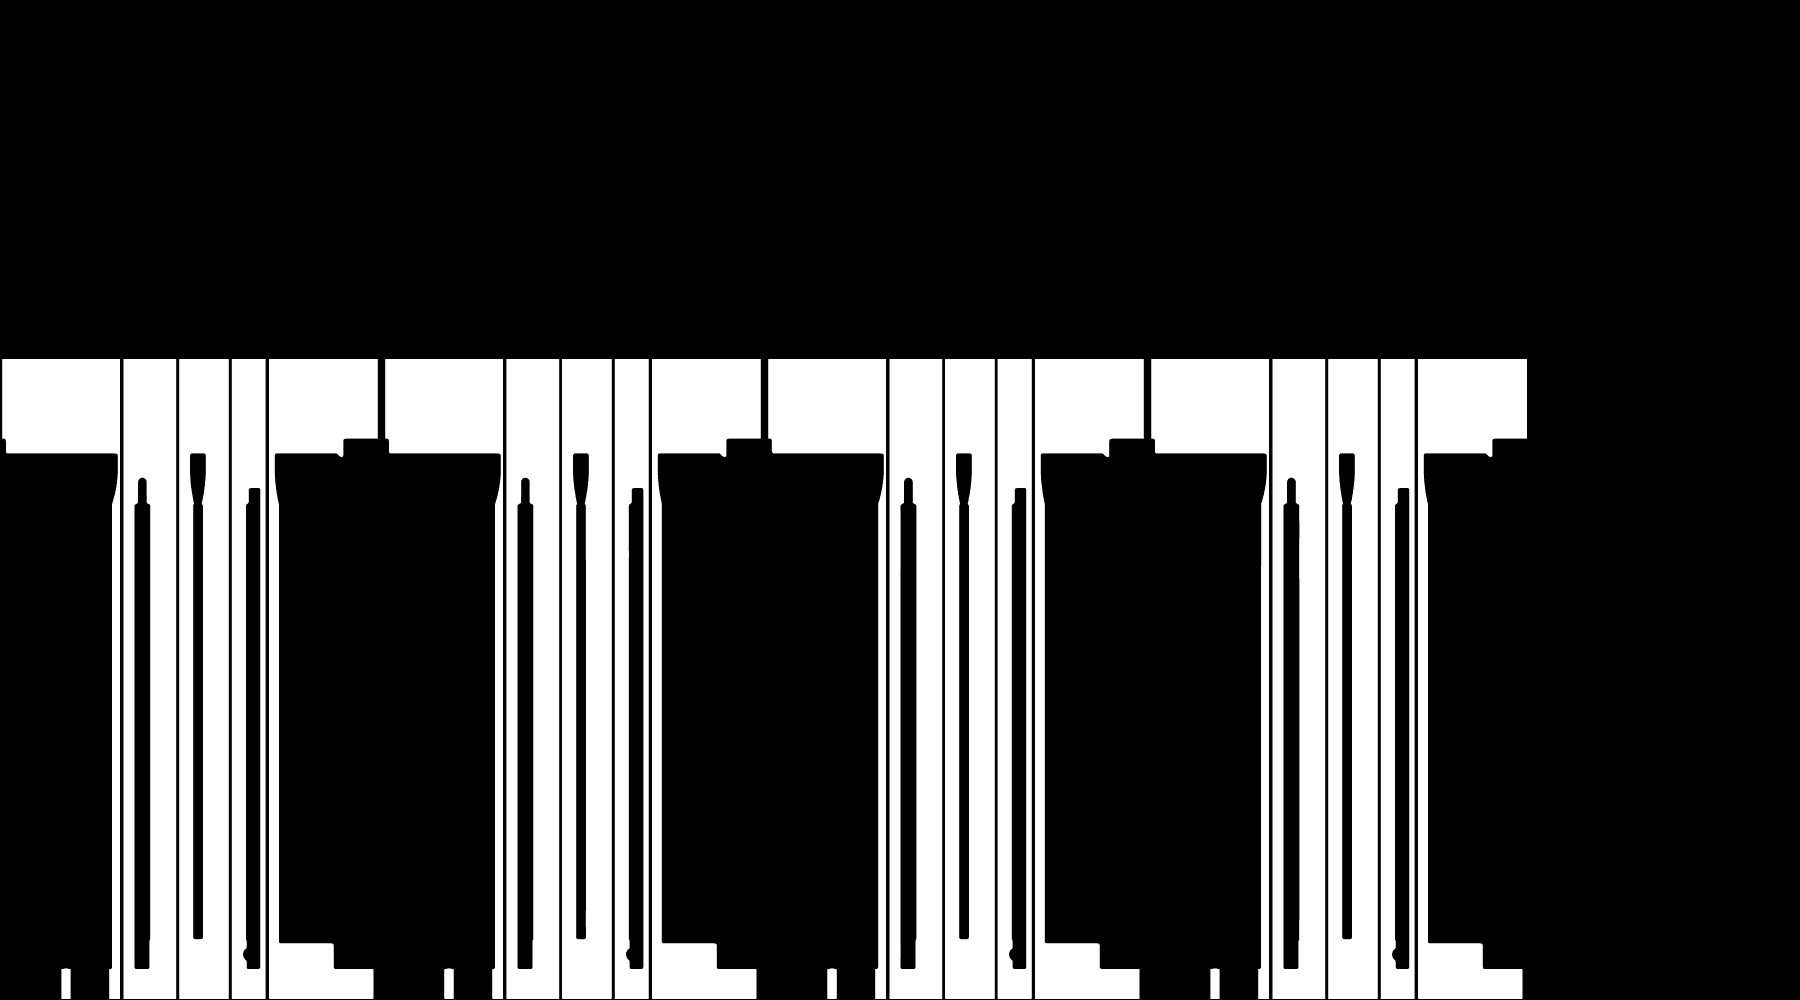
\includegraphics[width=\textwidth]{images/bitmask_01486}
    \caption{Corresponding bitmask must be checked to see if it's a scratch or a thin split.}
  \end{subfigure}

  \caption{Thin splits}
  \label{fig:thin_splits}

\end{figure}

The safer, but more tedious route is to check layer by layer the corresponding bitmask. This is only one of the many things to consider when annotating.\\

Sometimes the scratch is also barely visible or one cannot be sure if the scratch is relevant. Adding every fine scratch will make the model oversensitive, leading to many false positive. One statistical way to determine the strength of a labeled scratch goes roughly as follows:
\begin{enumerate}
\item Crop from the layer a window outlined by the bounding box.
\item Calculate the sum of rows of the image into a vector.
\item Multiply by -1 the whole vector.
\item Treat the vector as a signal and calculate prominences for the peak.
\item Multiple the prominence by a constant scaling factor.
\end{enumerate}

This way the bounding box is converted to signal, which makes a analysis of the strength of the scratch a bit more deterministic. After the 3rd step the plotted vector should look like this:

\begin{figure*}[!h]
\begin{center}
        \begin{subfigure}{0.3\textwidth}
        \centering
        
\includegraphics[width=0.2\textwidth]{images/crop_bb}
        \caption{Cropped bounding box}
    \end{subfigure}
                \quad
    \begin{subfigure}{0.55\textwidth}
        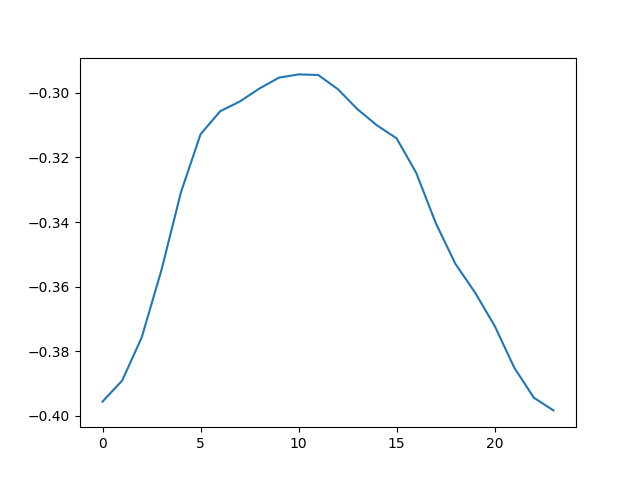
\includegraphics[width=\textwidth]{images/signal_bb}
        \caption{Bounding box signal}
    \end{subfigure}
            \quad

\caption{TODO: align images.  Transforming a bounding box to a signal.}
\label{default}
\end{center}
\end{figure*}

This method forces the annotation process to be more consistent, but it should be treated as statistical process and not as a deterministic one. In figure \ref{fig:prom_ex} can be seen why this process should not be seen as deterministic: the two scratches are of similar visibility, but have very different prominence values. Luckily, such outliers were rare. \\
One nice trick to visualize the scratches with the respective prominence value was to create a copy of the existing ground truth dataset and transform the ground truth labels to detections and as confidence value to use the prominence value. Note that in YOLOv5 the only difference between a ground truth bounding box and detection is that the detection has the optional confidence value filled out or less than 1.0. TODO: refer to the chapter that discusses labels (and also update that chapter) \\

\begin{figure}[!h]
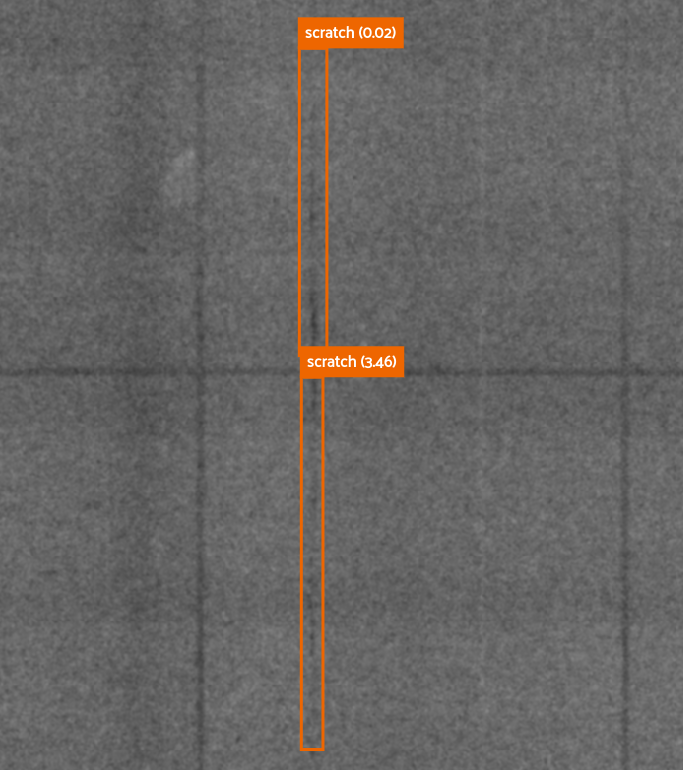
\includegraphics[width=\linewidth]{images/prominence_example}
\caption{Scratches with prominence values.}
\label{fig:prom_ex}
\end{figure}

Another problem are artifacts, that come from previous layers. Some cases are easy to recognize, but a common tricky situation is, if thin splits from previous layers are visible on the current layer. In those situations the thin splits might look like a scratch, have an acceptable prominence value and the bitmask indicates that in the respective region is no thin split. Therefore, the only way to really determine, if it's a scratch or not, is to analyze the previous layer too. As one can see, the annotation process got even more tedious, which means that data gathering is time-consuming and/or expensive.
TODO: say later we will see data cost table \\

\begin{figure*}[!h]
\begin{center}
        \begin{subfigure}{0.6\textwidth}
        \centering
        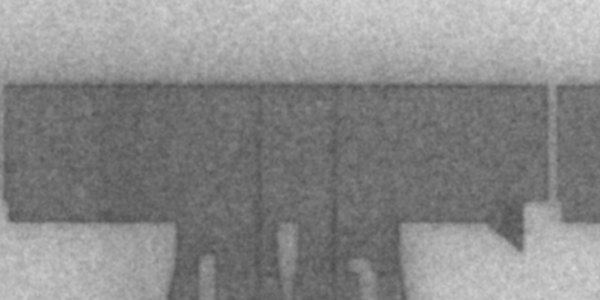
\includegraphics[width=\textwidth]{images/thin_scratch_previous_layer/layer_00107}
        \caption{A layer with dark lines}
    \end{subfigure}
                \quad
    \begin{subfigure}{0.6\textwidth}
        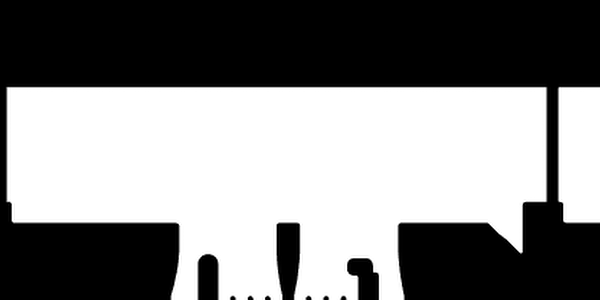
\includegraphics[width=\textwidth]{images/thin_scratch_previous_layer/bitmask_00107}
        \caption{Current bitmask has no splits.}
    \end{subfigure}
    \begin{subfigure}{0.6\textwidth}
        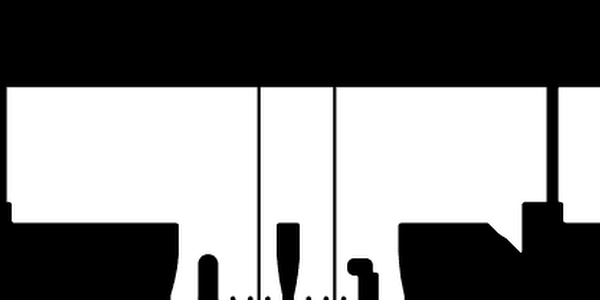
\includegraphics[width=\textwidth]{images/thin_scratch_previous_layer/bitmask_00106}
        \caption{Previous bitmask contains the seen splits.}
    \end{subfigure}
            \quad

\caption{Example of how thin splits are actually from the previous layer.}
\label{fig:thin_splits_previous_layer}
\end{center}
\end{figure*}

TODO train validation mixing \\
TODO border cutting \\


\subsection{Augmentation Pipeline}
TODO: muss ich sagen woher ideal dataset? \\
The dataset at hand features a total of 2295 images of layers with the corresponding bitmask, but only a fraction of the images contain an actual scratch. This makes the dataset from the recommended minimum of 1500 images per class and 10000 instances per class. This forced a focus shift on augmentation methods. \\
When it came to evaluating an augmentation method, identical dataset shuffles (train, validation, test splits) were used for multiple reasons. One reason is that it's easier to visually compare the validation errors, if the exact same image is used. One nice feature supported with Weights \& Biases logger is the Bounding Box Debugger, which lets the user see the validation labels for each epoch for multiple runs. If the runs had the exact same validation images, then a head-to-head comparison was possible.\\

\begin{sidewaysfigure}
    \centering
    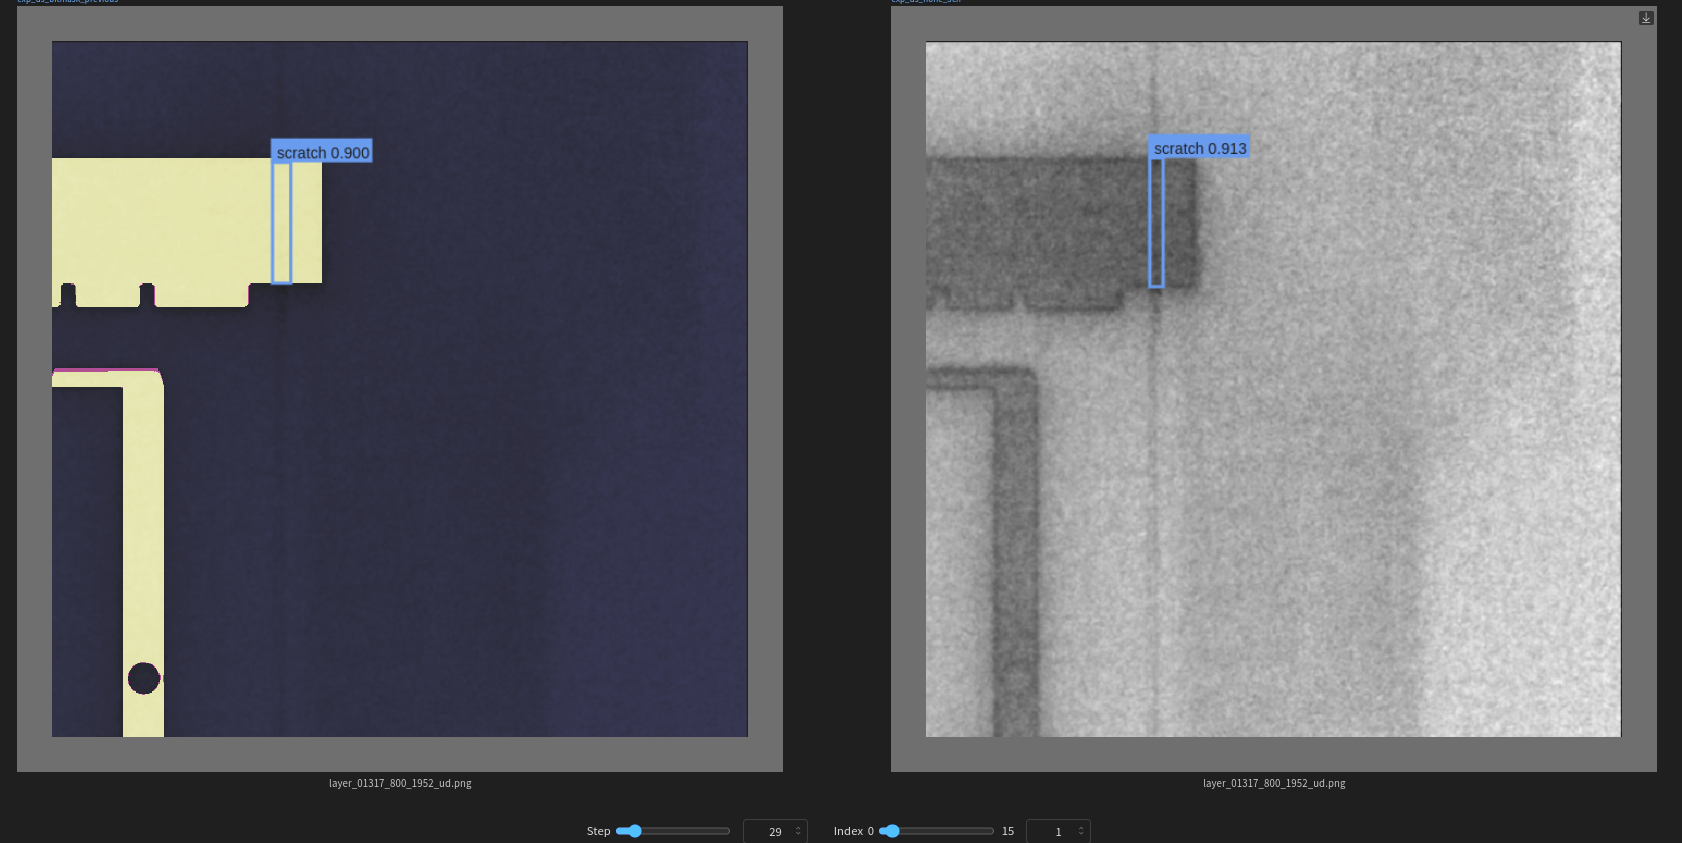
\includegraphics[width=\textwidth]{images/bb_debugger}
    \caption{Comparing head-to-head detections on validation images with the Bounding Box Debugger}
    \label{fig:bb_deb}
\end{sidewaysfigure}

Another reason for using identical shuffles is that in small datasets, shuffles are game of chance in terms of data variety. So, when using an identical shuffle, the same variety is ensured. TODO: maybe delete or reformulate this. \\


\subsection{Windowing}
One of the most analyzed and exhaustively tested augmentation method is the windowing method. This method simply takes a rolling window over the image and splits the images in smaller crops, called windows. First, some initial remarks will be presented.
\begin{itemize}
\item \textbf{Less CUDA memory:} The training process will now use smaller images, so there will more CUDA memory available, which means a bigger batch size is possbile.
\item \textbf{Bounding box conversion:} The bounding boxes need to be adjusted to the new window. Luckily, the albumentations library cropping methods supports this.
\item \textbf{Square vs rectangular training:} The initial intuition was to use tall rectangular windows, that can contain even the longer scratches. This way, the risk of obtaining tiny parts of a scratch in a window was avoided. However, YOLOv5 dataloader support shuffling only for square input images, which in some initial experiments showed a great improvement. Also, the cropping methods from albumentations support filtering tiny bounding boxes.
\item \textbf{Training times:} After splitting the data into windows, a lot of background windows (i.e. windows that do not contain scratches) are obtained, which can be filtered from the dataset. If not mentioned otherwise, all the background images/windows are removed from the dataset. This greatly improves training times by showing to the model only relevant sections of layers that contain scratches. YOLOv5 documentation recommends about 0-10\% background images. Also, images of smaller resolution take less time to be processed.
\item \textbf{Window overlapping:} In some unlucky cases a scratch might land on the edge of a window. To avoid this situation, all neighbouring windows have an overlap between them.
\end{itemize}

\subsubsection{Windowing Strategy}
The first window strategy, called \textit{grid windowing}, used to extract windows at the same positions for each layer. This showed great results, but a potential problem was that some consecutive layers had the scratches at the exact same locations. This lead to the development of \textit{random windowing}, which crops 1-2 random windows containing each scratch. In this way, the series of similar layers with repeating scratches was diversified into windows that contained the scratches at different positions. However, this method was sometimes unstable. The key difference is that at \textit{grid windowing} a scratch could be captured in 2 neighboring windows due to the overlap and this way the same scratch was captured in twice but at different positions at the window. At \textit{random windowing} this effect could be simulated by taking a random window of the scratch twice, but there was no guarantee that the windows capture the scratch in 2 different perspective. The randomness of this strategy could of course be improved, but it was not worth the effort since \textit{grid windowing} does it good enough. TODO explain better. TODO insert image explaining this concept. In figure \ref{fig:win_strategy} the windows of both methods can be visualized.  TODO: maybe try on second dataset.

\begin{figure}
  \begin{center}
  \begin{tabular}{ c c c }
  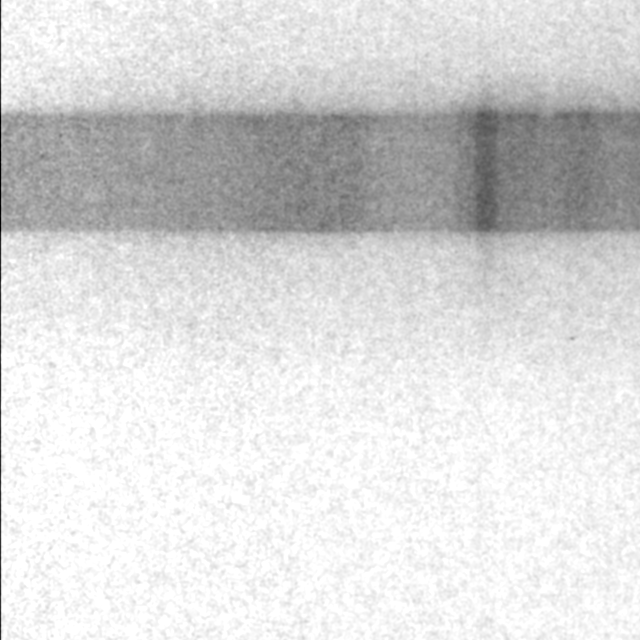
\includegraphics[width=.3\linewidth]{images/win_strategy/layer_21_grid} &
  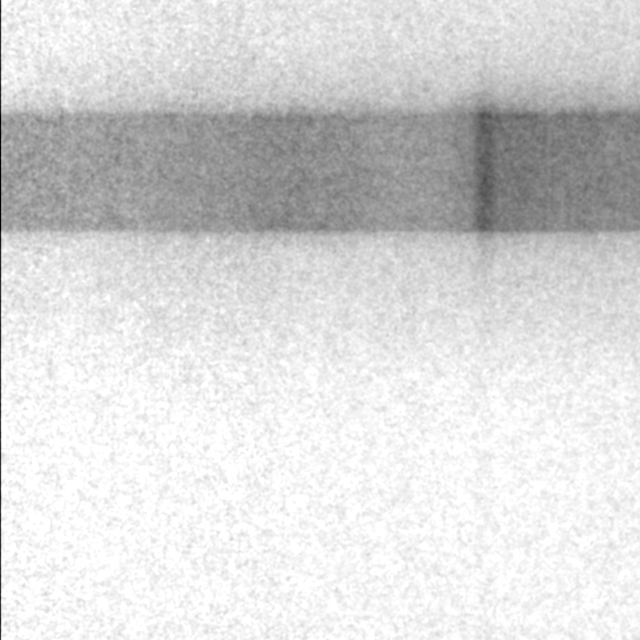
\includegraphics[width=.3\linewidth]{images/win_strategy/layer_22_grid} &
  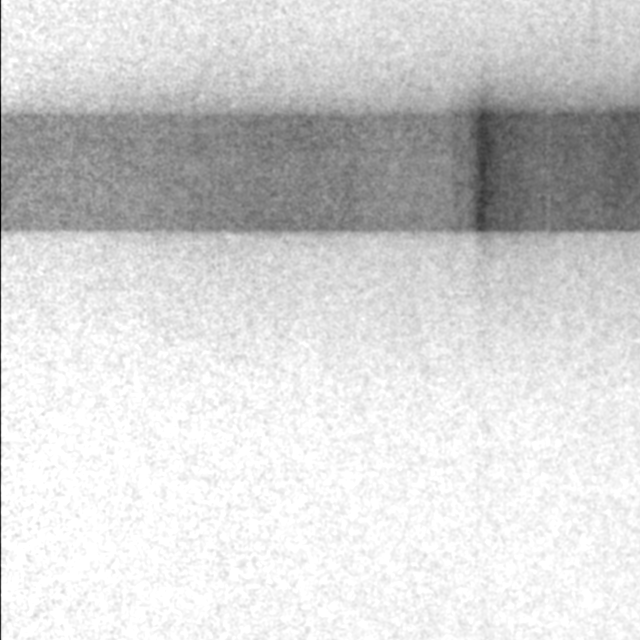
\includegraphics[width=.3\linewidth]{images/win_strategy/layer_23_grid} \\
   & & \\
  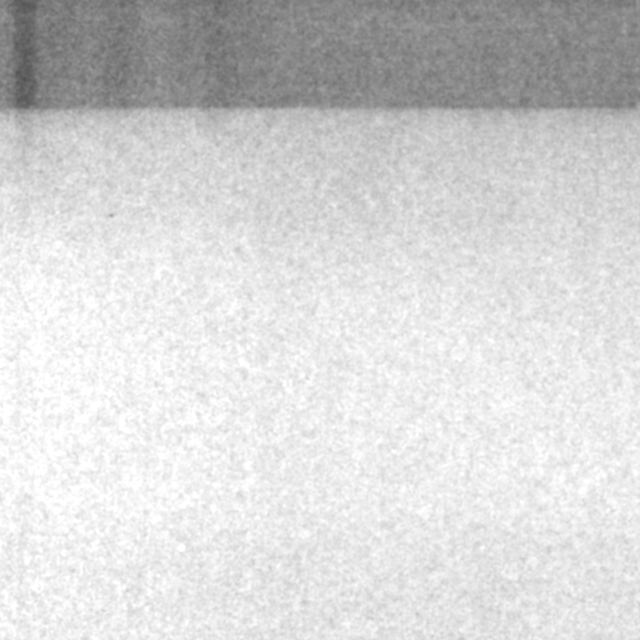
\includegraphics[width=.3\linewidth]{images/win_strategy/layer_21_rand} &
  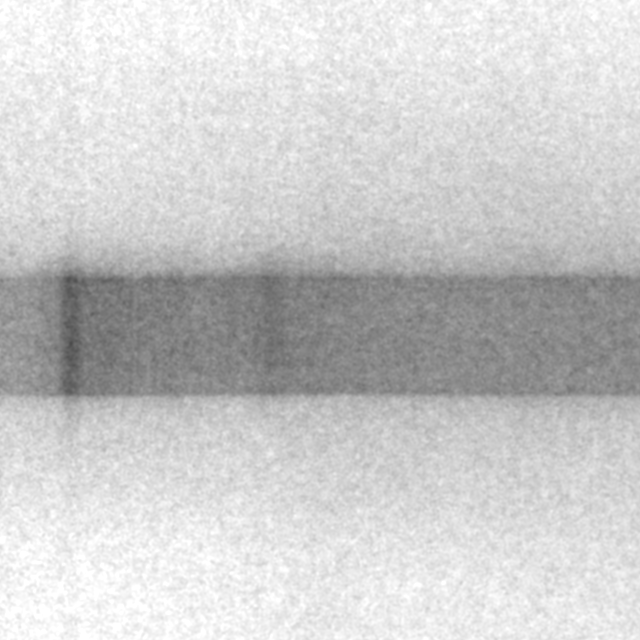
\includegraphics[width=.3\linewidth]{images/win_strategy/layer_22_rand} &
  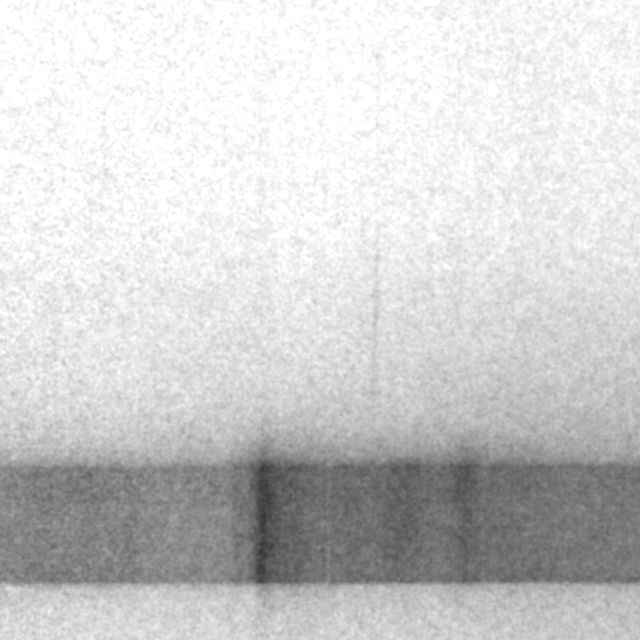
\includegraphics[width=.3\linewidth]{images/win_strategy/layer_23_rand} \\
  \end{tabular}
  \end{center}

  \caption{An exmample of the windowing strategies on 3 similar layers with repeating scratches. The first row shows the grid windowing method and the second row shows the random windowing method.}
  \label{fig:win_strategy}
\end{figure}

\subsubsection{Window Size}
For testing the effects of the window size, YOLOv5 has been trained on datasets with window sizes of 320, 640, 960 and 1280. The single constraint imposed by YOLO detectors is that the height and width needs to be a multiple of 32. \\
When it comes to better metrics, bigger windows got the better results. The intuitive explanation is that a bigger window may contain not only the annotated scratch itself, but also other dark lines that mimic a scratch like the thin splits shown in figures \ref{fig:thin_splits}, \ref{fig:thin_splits_previous_layer}.\\

\begin{figure}
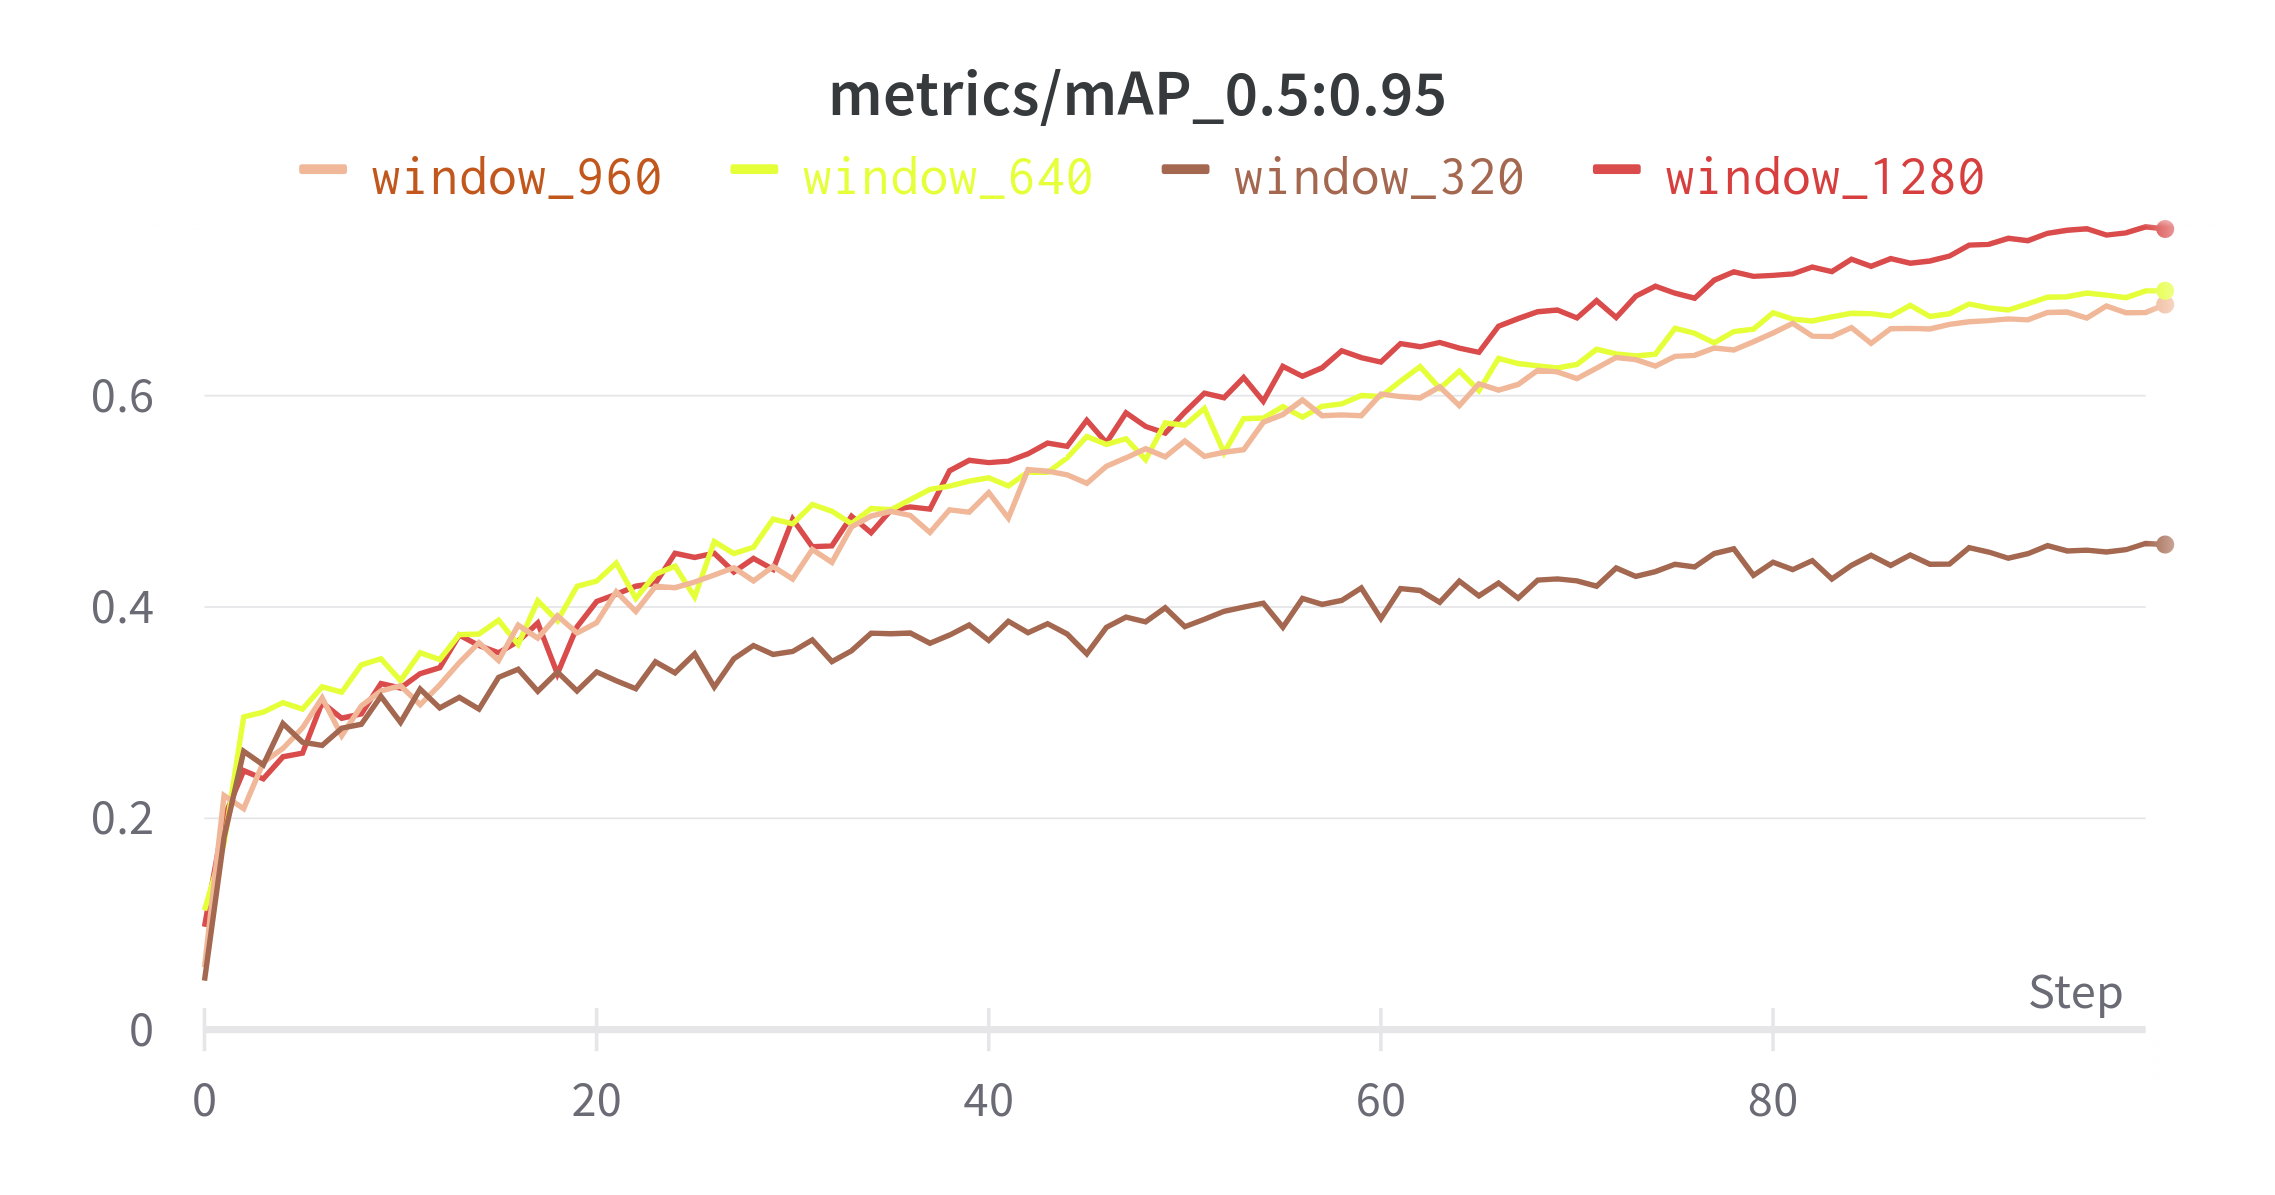
\includegraphics[width=\textwidth]{images/map_win_size}
\caption{mAP@0.5:0.95 for different window sizes}
\end{figure}

 Bigger windows might have the advantage of capturing more context information, but the drawback is the longer training time as seen in figure \ref{fig:win_train_times}. One naive way to add more context information is to simply keep more background windows with the hope of capturing informative backgrounds, but multiple experiments with different percentage of backround images did not improve the metrics. The problem was that only background images of printed surface have the potential to teach the model something relevant and keeping random background images in the dataset proved not help in any way. With this mind, a new way of keeping background information has been found: Let's say that the desired window size is 320x320. First a dataset \textit{A} with window size of 640x640 is generated and all the background windows are removed. After that, a dataset \textit{B} is obtained by spliting each window from dataset \textit{A} in 4 smaller 320x320 windows. This time all the background windows are kept. The general idea is that it is more likely to find printed regions near a scratch. Training on this new dataset B takes on average 2-3 times longer to train than on a simple 320x320 dataset with 0-10\% background images. \\

\begin{figure}
  \begin{tabular}{|c|c|}
  \hline
  window size & epoch time (in seconds) \\
  \hline
  320x320 & 16 \\
  \hline
  640x640 & 35 \\
  \hline
  960x960 & 40 \\
  \hline
  1280x1280 & 102 \\
  \hline
  \end{tabular}
  \caption{Epoch time for the same dataset, but with different window sizes.}
  \label{fig:win_train_times}
\end{figure}


 One interseting fact for this approach was that training on dataset \textit{B} produced metrics very close to ones from training on dataset \textit{A}. This concept was tested on multiple window sizes for consistency. \\


 \subsubsection{Rectangular training and other caveats}
 TODO
with --rect no shuffling, image padded, no mosaic or cut-mix



\subsection{Mosaic and Cut-Mix}


\subsection{Translate and Scale}

\subsection{Create Custom Online Augmentation}

\subsection{Stretches and Squeezes}
Luckily the presented dataset had generally a good distribution of the lengths of scratches, but an interesting research topic was the robustness of the trained model.
TODO plot distribution \\

 How well does YOLOv5 perform at detecting longer scratches, if it was trained only on shorter scratches? And vice-versa? A


TODO talk about artifical examples?? \\

\subsubsection{Constrast}



\subsection{Hyperparameter Optimizations}

\subsubsection{Model Size}

\subsubsection{Hyperparameter evolution}

\subsubsection{Batch Size}
The official documentation recommends that training should be performed on the biggest batch size possible in order to produce the best batch normalization statistics, but meanwhile on the official Github repository the developers suggest that YOLOv5 is batch agnostic (TODO source). For the sake of finding the truth, multiple experiments with varying batch sizes have been made. The results were that for batch sizes up to 64 the map@0.5:0.95 metric was in favour of bigger batch sizes. Other metrics had no tangible differences. Bigger batches required more than 2 GPUs or compromising to a smaller window size. \\
TODO show results \\

\subsubsection{Learning Rate and Gradient}
The initial experiments showed high jumps after each epoch, so a switch from the standard stochastic gradient descent to AdamW has been made. The documentation recommends for AdamW to change the learning rate from 0.01 to 0.001, but a step size of 0.0001 showed a more stable evolution from epoch to epoch.
TODO maybe show some results

\subsubsection{Loss Function}


\subsubsection{IoU threshold}


TODO obiective dataset:
scratches position
scratches length should have variety (prin stretch si prin window cuts)
scratch strength variety (sa inventez ceva)

easy source code modifications (la metrics mai ales)
dataset format
dataset postprocessing (black border)
